\chapter{Obsah CD}
Adresárová štruktúra CD
\begin{itemize}
\item Zdrojové súbory
    \begin{itemize}
    \item Webový portál
    \item Javascriptové API
    \item Hra
    \item Databázový skript
    \end{itemize}
\item Grafika
\item Text
\end{itemize}

\chapter{Dokumentácia k API}

\chapter{Ukážky z implementácie}
\begin{figure}[h]
  \centering
  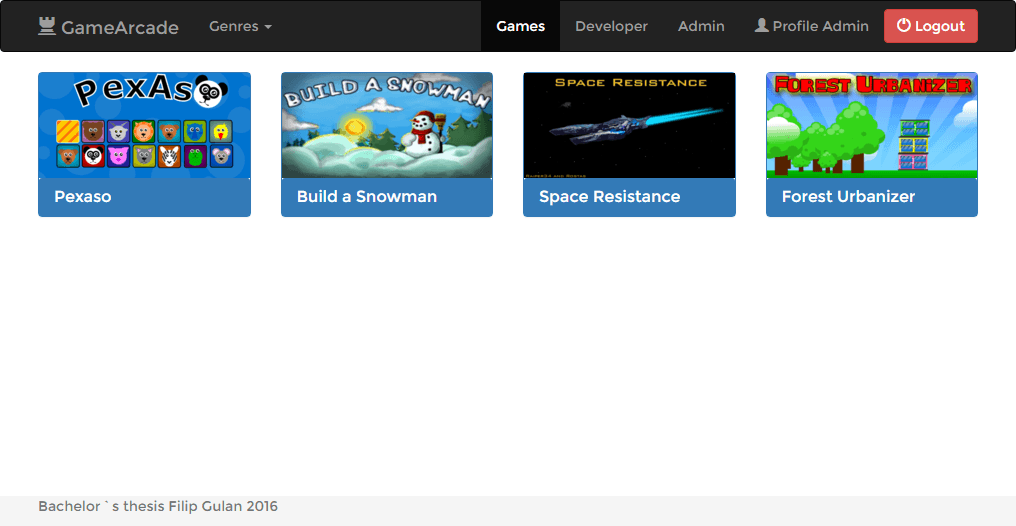
\includegraphics[scale=0.35]{fig/ukazka-zoznam-hier.png}
  \caption{Ukážka obrazovky so zoznamom hier. Hore na lište vedľa textového loga sa nachádza filtrovanie podľa žánru.}
  \label{fig:ukazka-zoznamhier}
\end{figure}

\begin{figure}[h]
  \centering
  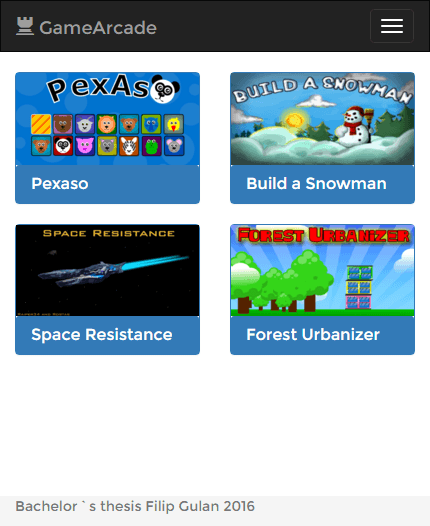
\includegraphics[scale=0.35]{fig/ukazka-responzivity.png}
  \caption{Ukážka zoznamu hier a jeho responzívnosti.}
  \label{fig:ukazka-zoznamhierresponzivny}
\end{figure}

\begin{figure}[h]
  \centering
  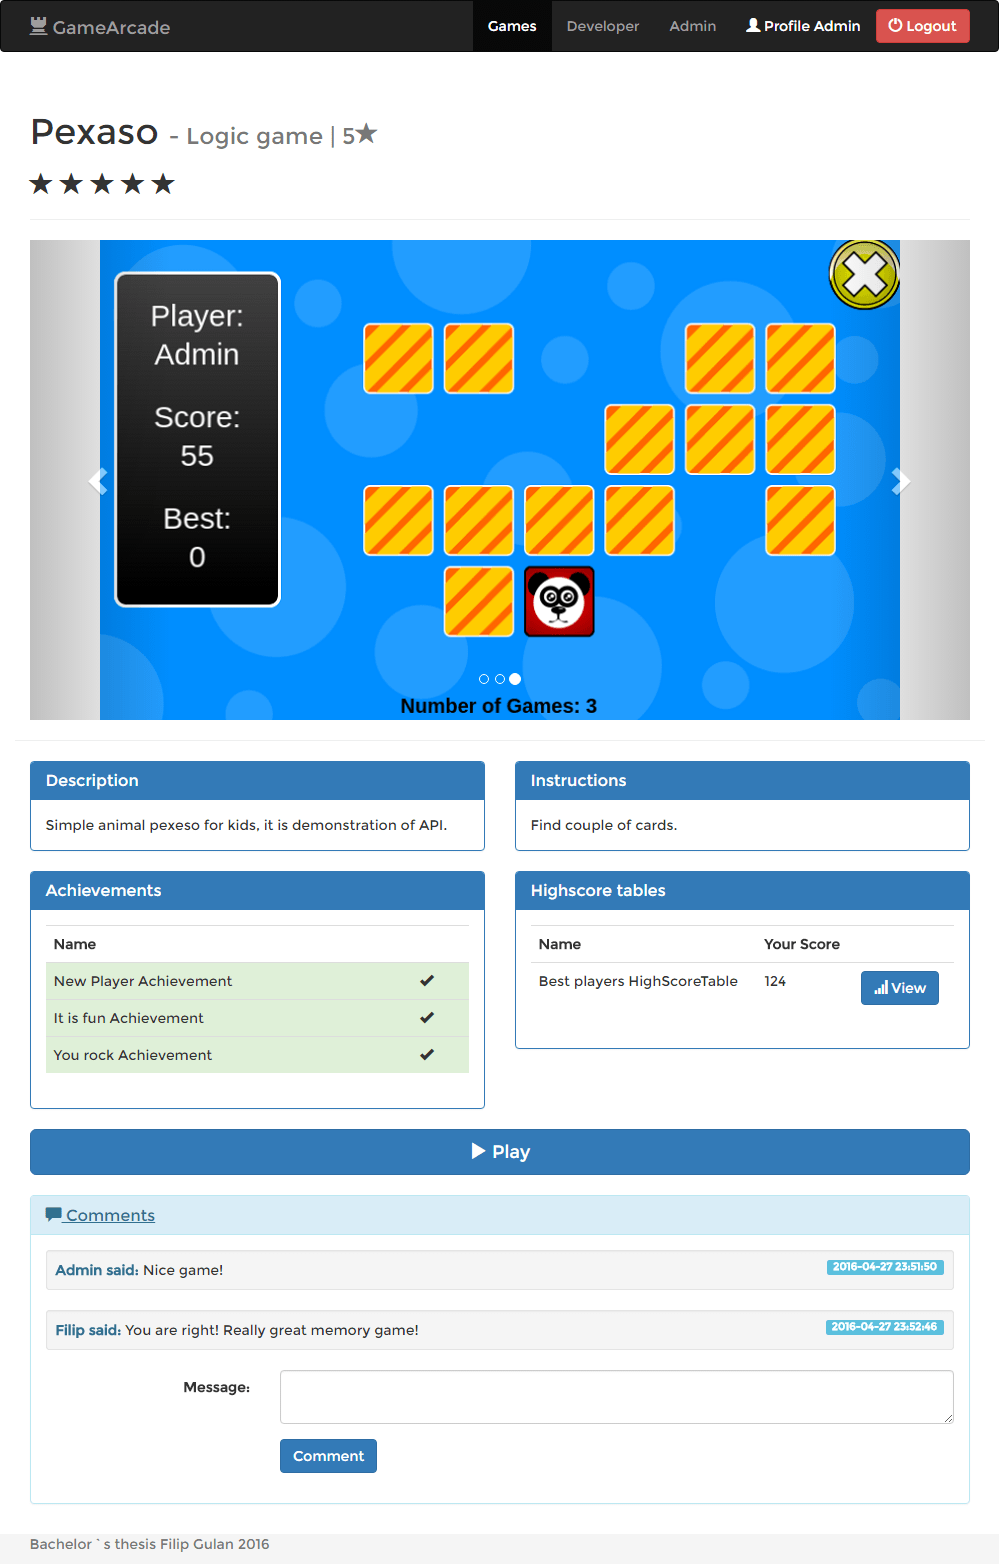
\includegraphics[scale=0.35]{fig/ukazka-detail-hra.png}
  \caption{Ukážka detailu hry. Nachádzajú sa tu panely s s jednotlivými informáciami (napríklad panel s odmenami, tabuľkami...)}
  \label{fig:ukazka-detailhry}
\end{figure}

\begin{figure}[h]
  \centering
  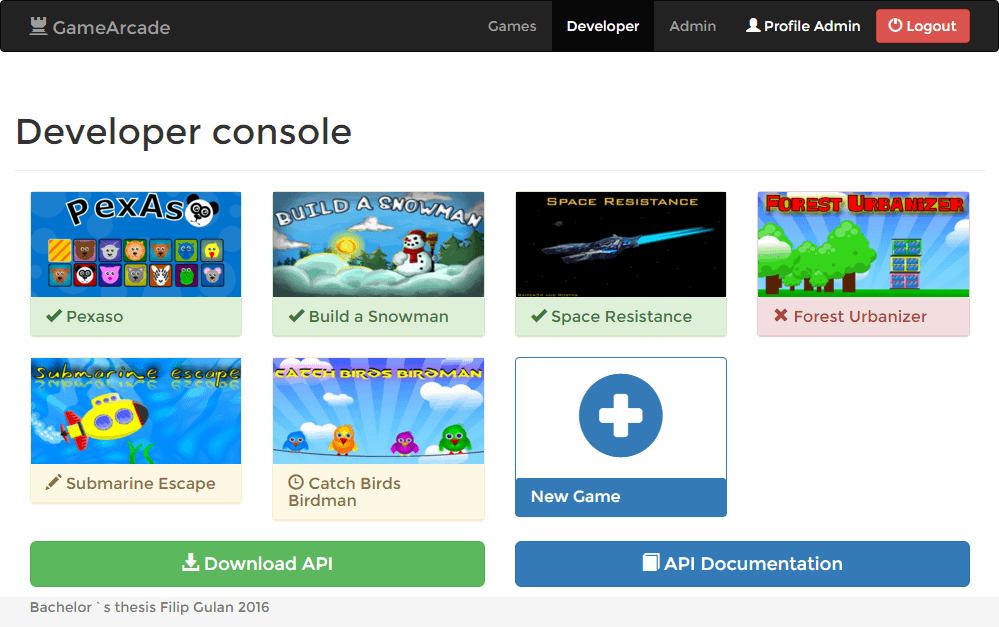
\includegraphics[scale=0.35]{fig/ukazka-zoznam-vyvojar.png}
  \caption{Ukážka vývojárskej konzole. Je možné vidieť hry v rôznom štádiu publikácie, ktorých panely sú farebne odlíšené.}
  \label{fig:ukazka-vyvojar}
\end{figure}

\begin{figure}[h]
  \centering
  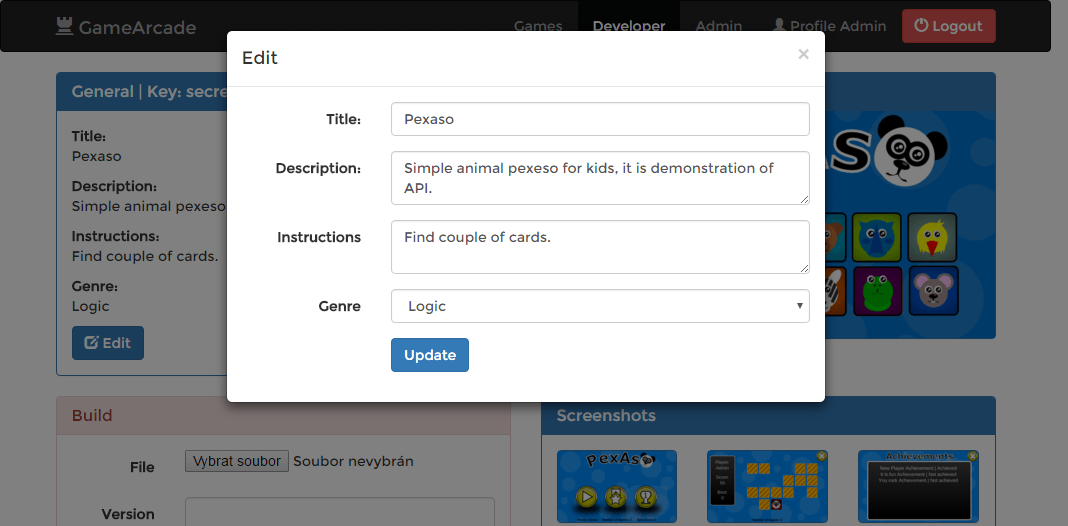
\includegraphics[scale=0.35]{fig/ukazka-modalne-okno.png}
  \caption{Ukážka úpravy informácií v detailu hry vo vývojárskej konzoly pomocou modálneho okna.}
  \label{fig:ukazka-modalneokno}
\end{figure}

\begin{figure}[h]
  \centering
  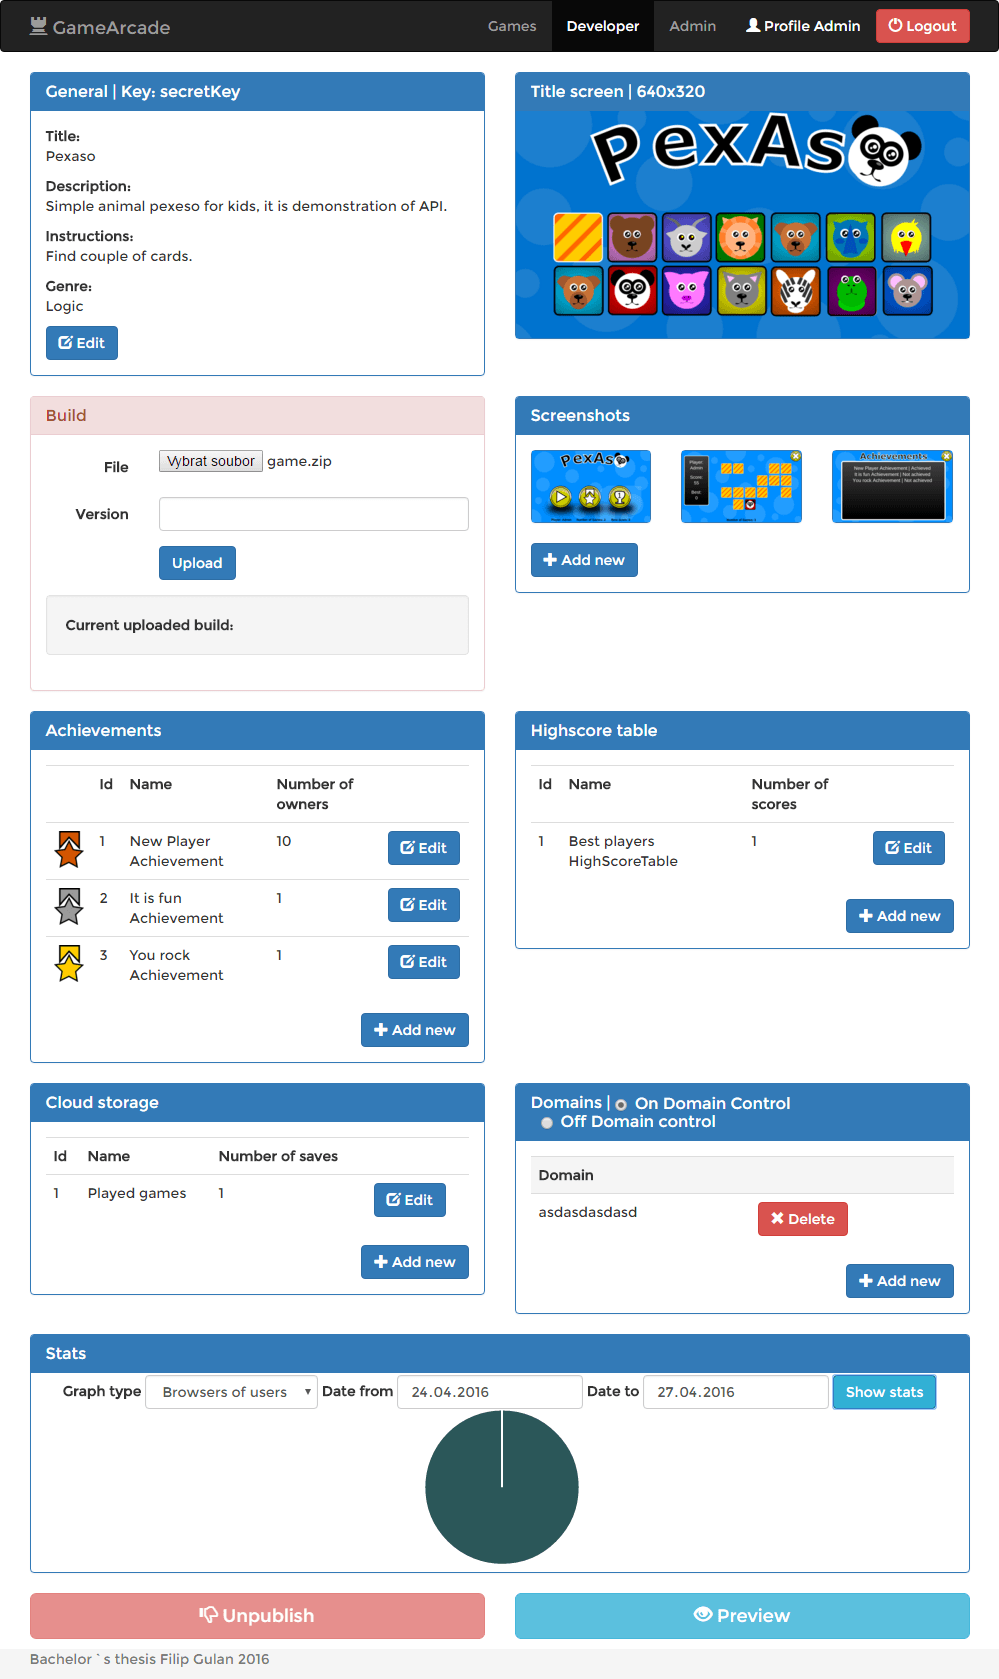
\includegraphics[scale=0.35]{fig/ukazka-detail-vyvojar.png}
  \caption{Ukážka detailu hry vo vývojárskej konzoly. Je možné vidieť jednotlivé panely, ktoré logicky oddeľujú jednotlivé informačné a editačné sekcie.}
  \label{fig:ukazka-detialvyvojar}
\end{figure}

\begin{figure}[h]
  \centering
  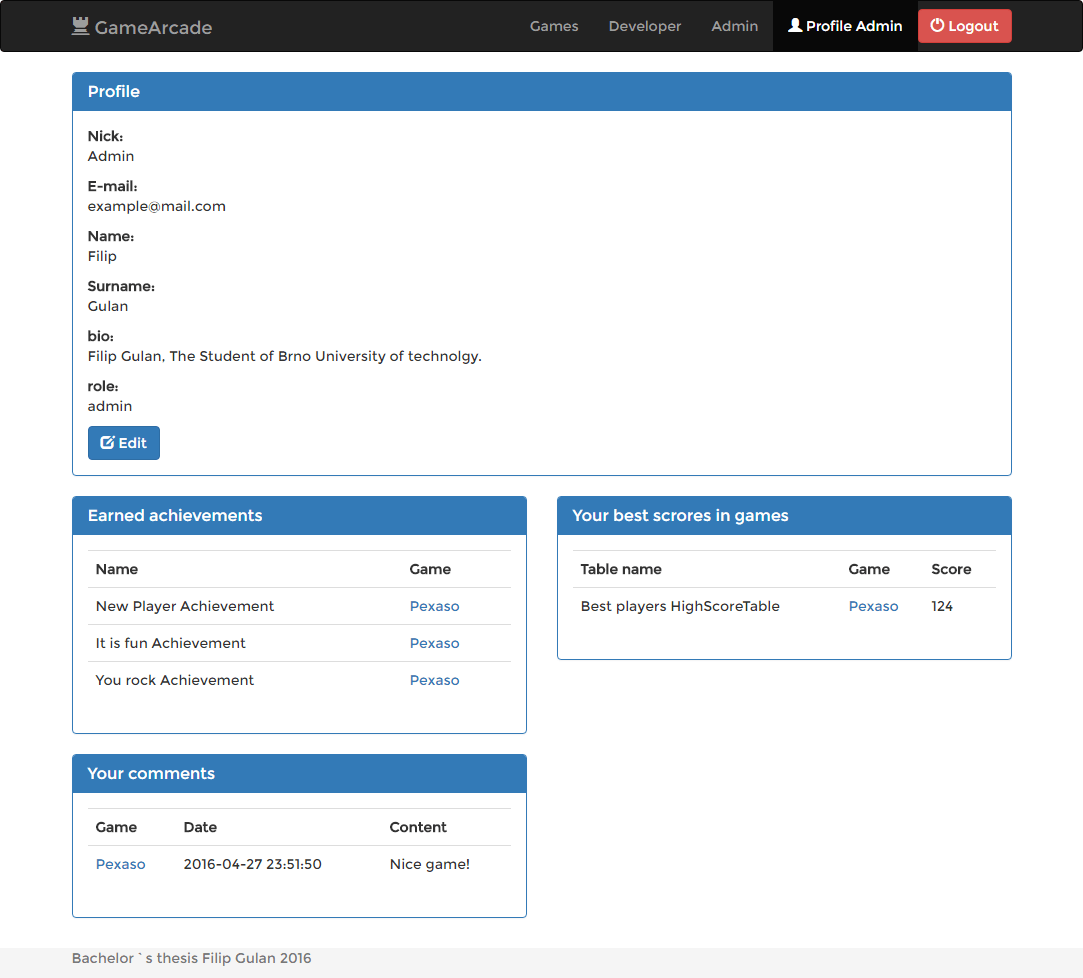
\includegraphics[scale=0.33]{fig/ukazka-profil.png}
  \caption{Ukážka profilu užívateľa.}
  \label{fig:ukazka-profil}
\end{figure}

\begin{figure}[h]
  \centering
  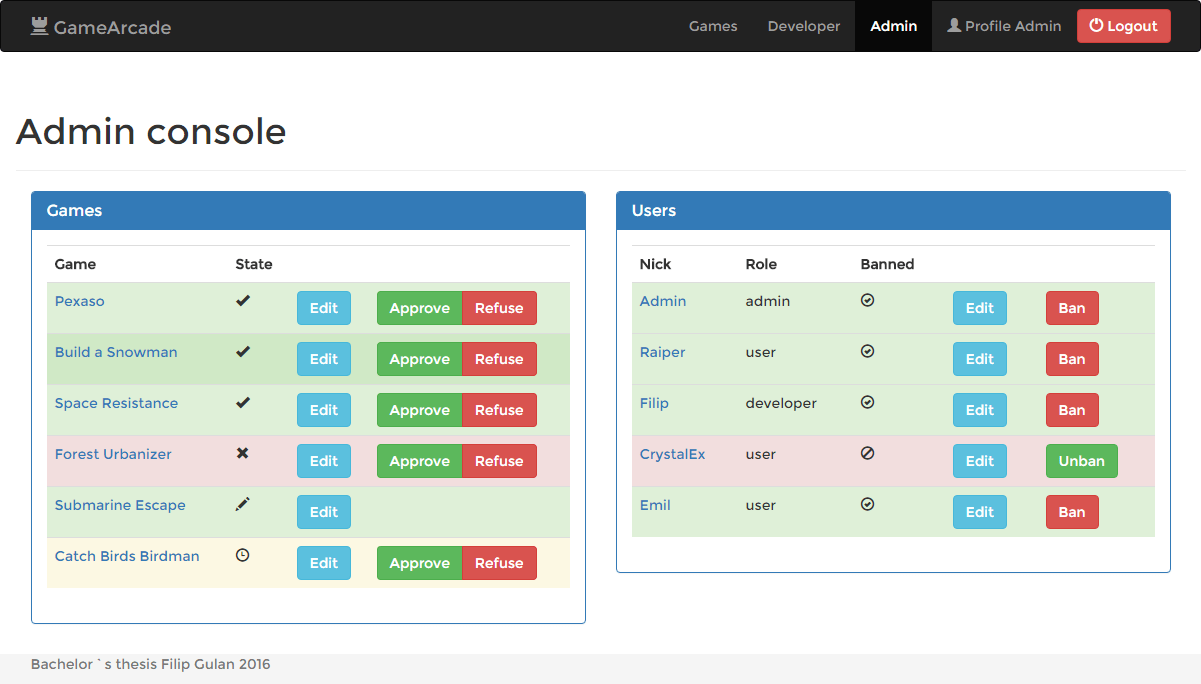
\includegraphics[scale=0.35]{fig/ukazka-admin.png}
  \caption{Ukážka administrátorskej konzoly. Je možné vidieť farebne odlíšené hry v jednotlivých štádiách publikácie a užívateľov, taktiež farebne odlíšených, podľa toho, či sú povolený, alebo zakázaný.}
  \label{fig:ukazka-admin}
\end{figure}

\begin{figure}[h]
  \centering
  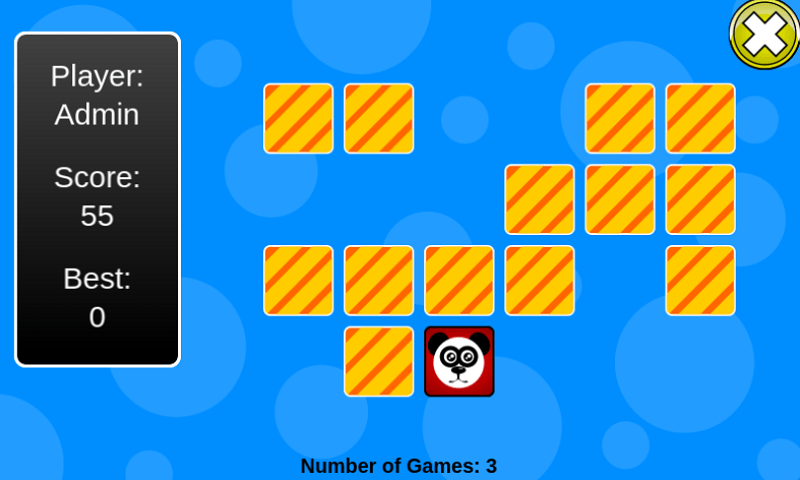
\includegraphics[scale=0.45]{fig/ukazka-hra.png}
  \caption{Ukážka levelu v demonštračnej hre. Naľavo je možné vidieť informačný panel, s informáciami, ktoré sú získané zo serveru pomocou implementovaného API.}
  \label{fig:ukazka-hra}
\end{figure}

\begin{figure}[h]
  \centering
  
\includegraphics[scale=0.45]{fig/ukazka-hra-odmeny.png}
  \caption{Ukážka hernej obrazovky s odmenami. Obsahuje meno domény a informáciu o tom, či ju aktuálne prihlásený užívateľ získal.}
  \label{fig:ukazka-hraodmen}
\end{figure}



